\documentclass[12pt]{article}
\setlength\parindent{0pt}
\usepackage{fullpage}
\usepackage[margin=0.5in, paperwidth=13.5in, paperheight=8.4375in]{geometry}
\usepackage{amsmath}
\usepackage{graphicx}
\setlength{\parskip}{4mm}
\def\LL{\left\langle}   % left angle bracket
\def\RR{\right\rangle}  % right angle bracket
\def\LP{\left(}         % left parenthesis
\def\RP{\right)}        % right parenthesis
\def\LB{\left\{}        % left curly bracket
\def\RB{\right\}}       % right curly bracket
\def\PAR#1#2{ {{\partial #1}\over{\partial #2}} }
\def\PARTWO#1#2{ {{\partial^2 #1}\over{\partial #2}^2} }
\def\PARTWOMIX#1#2#3{ {{\partial^2 #1}\over{\partial #2 \partial #3}} }
\newcommand{\BE}{\begin{displaymath}}
\newcommand{\EE}{\end{displaymath}}
\newcommand{\BNE}{\begin{equation}}
\newcommand{\ENE}{\end{equation}}
\newcommand{\BEA}{\begin{eqnarray}}
\newcommand{\EEA}{\nonumber\end{eqnarray}}
\newcommand{\EL}{\nonumber\\}
\newcommand{\la}[1]{\label{#1}}
\newcommand{\ie}{{\em i.e.\ }}
\newcommand{\eg}{{\em e.\,g.\ }}
\newcommand{\cf}{cf.\ }
\newcommand{\etc}{etc.\ }
\newcommand{\Tr}{{\rm tr}}
\newcommand{\etal}{{\it et al.}}
\newcommand{\OL}[1]{\overline{#1}\ } % overline
\newcommand{\OLL}[1]{\overline{\overline{#1}}\ } % double overline
\newcommand{\OON}{\frac{1}{N}} % "one over N"
\newcommand{\OOX}[1]{\frac{1}{#1}} % "one over X"



\begin{document}
\pagenumbering{gobble}
\Large
\centerline{\sc{Recitation Questions -- March 13}}
\normalsize
\begin{enumerate}

	\item{Someone drops a penny of mass 2.5g off of the Empire State Building (height 380 m). It strikes the ground traveling at 50 m/s, having been slowed somewhat by air drag.}
\begin{enumerate}
	\item{With what velocity would it have struck the ground if there were no air resistance?}
	
	\vspace{1.5in}
	
	\item{What was the work done by the drag force?}
	
	\vspace{1.5in}
	
	\item{This penny strikes the sidewalk and penetrates the surface, digging a hole 2 cm deep. What was the upward force exerted on the penny by the pavement? {\it (Note: Think carefully about whether you need to worry about the work done by gravity on the penny as it moves another 2 cm.)}}
	
	\vspace{2in}
	
\end{enumerate}
\newpage

\item{My laptop battery says it has a capacity of 97 ``watt-hours''.}
\begin{enumerate}
	\item{What are the dimensions of this odd unit ``watt-hour'', and what does it measure? What is 97 watt-hours in more familiar units?}
	
	\vspace{2.5in}
	
	\item{My laptop has a mass of 2 kg. If it contained a motor instead of computing hardware, how far could its battery lift it (moving at constant velocity)?}
	
	\vspace{2.5in}
\end{enumerate}
\newpage
%
%\item {A rock climber of mass 70 kg is climbing a cliff face when she slips and falls. They are 2 meters above their last anchor, so they undergo free fall for 4 meters before the rope begins to arrest their fall. If the stiffness in their rope is 1400 N/m, then:}
%\begin{enumerate}
%	\item{How far will they fall in total?}
%	
%	\vspace{3in}
%	
%	\item{What is the maximum force that their rope will exert on them as it arrests their fall? Where does this maximum force occur?}
%	
%	\vspace{3in}
%\end{enumerate}
%\newpage

\it This next problem also appears on your homework. If you finish it here, you may submit this for homework.

\rm

\item Our former Physics 211 head TA Ohana Benevides is sitting on a tree swing, consisting of a light platform suspended by two ropes of length $L$. Her exceptionally friendly dog Rum (pronounced ``room''), who is half her mass and far too big to be a lap-dog but doesn't know it, runs toward her and then jumps in her lap.

The impact of the dog causes her to recoil backwards, and the swing swings upward to an angle $\theta$ before coming back down.

\begin{enumerate}

\item Draw cartoons of three relevant moments in time: (i) right before Rum lands in her lap, (ii) right after he lands in her lap, and (iii) when the swing is at its highest point. Label relevant things, in particular the velocities
of moving objects.

\vspace{3.5in}

\newpage

\item What physical principle can you use to relate the velocity of the dog before he jumps in her lap in cartoon (i) to the velocity of the person plus dog afterwards in cartoon (ii)?

\vspace{1in}

\item What physical principle can you use to relate the velocity of the person and dog in cartoon (ii) to the swing angle $\theta$ in cartoon (iii)?

\vspace{1in}

\item Using the principle you identified in (b), find a relation between Rum's initial velocity and the velocity of Rum and Ohana after he jumps in her lap.

\vspace{2in}
\newpage


\item What is the work done by gravity during the motion here? You will need to think carefully about geometry.

\vspace{3in}

\item How fast was Rum running when he jumped in her lap? Find an answer in terms of $L$, $\theta$, and $g$.



\end{enumerate}

\newpage

\begin{minipage}{0.5\textwidth}
\begin{center}
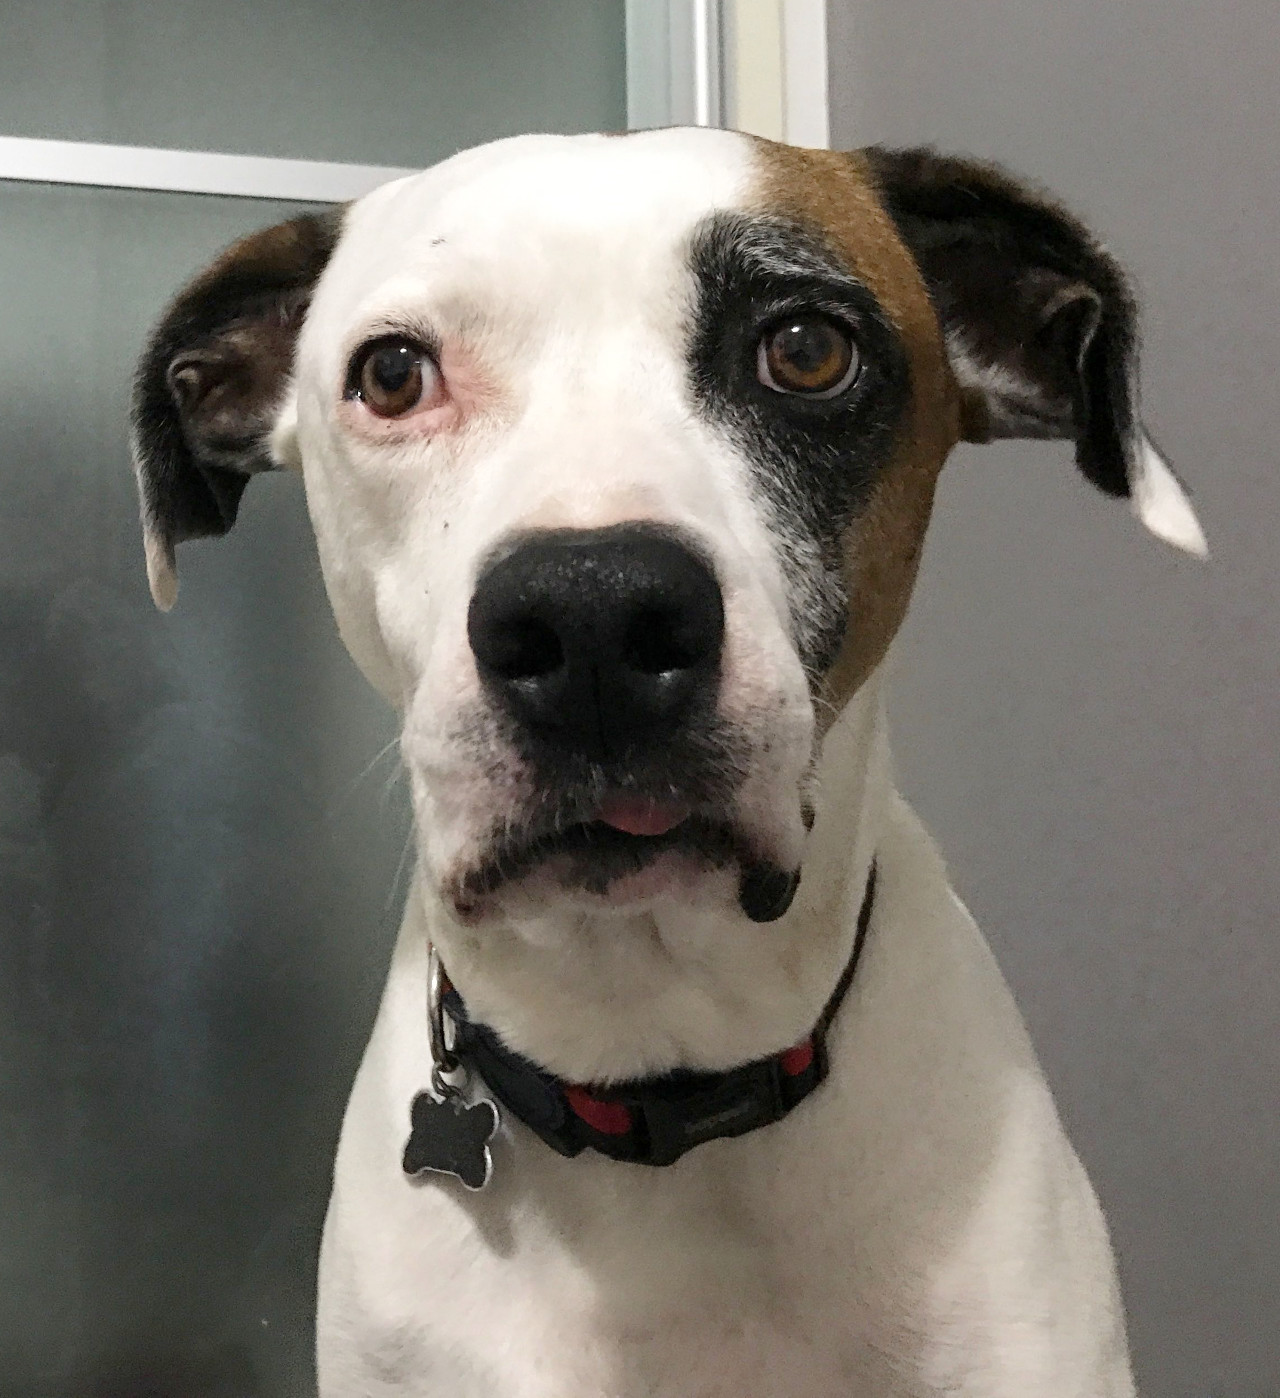
\includegraphics[width=\textwidth]{rum.jpg}\\
\scriptsize blep.
\end{center}
\end{minipage}
\begin{minipage}{0.5\textwidth}
\begin{center}
Rum the Physics Dog wants you to study hard. 

\bigskip
 Unless you have snacks for him. 
\bigskip

 Then he wants snacks.
\end{center}
\end{minipage}
\newpage

%\item A firecracker is launched straight upward. It is traveling upward at 30 m/s when it explodes, fracturing into two pieces. The larger piece is twice as massive as the smaller piece; after the explosion, it is traveling horizontally at 50 m/s.
%What is the velocity of the smaller piece after the explosion? Give its magnitude and direction.

\newpage






%\item A Yo-Yo consists of a cylinder of mass $m$ and radius $r$. A thin slot is cut in the middle of the cylinder such that the inner radius is only $r_{\rm in}=0.4r$, and a string is wound around the middle. (If you don't know what a Yo-Yo is, there is an animation on Wikipedia.) The moment of inertia of a cylinder is $I=\frac{1}{2}mr^2$. Suppose that a Yo-Yo has a string of length $L=1.2$ m, and its handler winds up the string, holds one end, and then drops the Yo-Yo. It will fall, unwinding its string,
%until it falls 120 cm and runs out of string.

%In this problem, you'll use the conservation of energy to find how fast the Yo-Yo is moving when it reaches the bottom.

%\begin{enumerate}

%\item Write down the work-energy theorem for the Yo-Yo as it falls. Note that the tension here does no work; there are several explanations for why, but the one based on the things that you know so far is that the {\it string is stationary}. 
%The point of contact between the string and the Yo-Yo doesn't slip; you can think of the spool ``rolling down'' the string, much like a ball rolls down a hill.

%\vspace{3.5in}

%\item What is the relation between the angular velocity $\omega$ and the translational velocity $v$ of the Yo-Yo? Call your TA/coach over to check your work on this part.

%\vspace{3.5in}

%\newpage

%\item Find its velocity when it reaches the bottom. Compare this to the velocity of an object that has been simply {\it dropped} the same distance.

%\vspace{3.5in}

%\item Does the slot in the middle of the Yo-Yo simply keep the string from sliding out, or does it serve some other purpose? Explain this to your TA/coach.

%\end{enumerate}
\end{enumerate}

\end{document}
 


